%!TEX root = ../SciVis.tex
\subsection{Skeleton compilation}
\subsection{Color mapping}


understand and implement a set of color mapping techniques for the fluid flow simulation

three datasets: The fluid density rho, the fluid velocity magnitude | v |, and the force field magnitude | f |

\ref{fig:rainbowColormap}
lookup table

color interpolation

how to specify a colormap
parameterization of colormap (hue and saturation) \ref{fig:saturationAndHueColormap}

defined colormaps \ref{fig:colormaps}
 
vertex vs texture

transform (linear or logarithmic)



banding 

legend  The legend should show both the colormap and the corresponding numerical values associated to various colors.


scaling: the entire actual range (min..max) of the dataset at the current time moment is mapped to the visible colormap. This means, of course, that you have to update the numerical values displayed along with the color legend.

clamping: the data values are clamped between two user-prescribed min and max values. These values correspond to the entire range of your color legend. Actual data values higher than min, or lower than max, are actually clamped to min and max respectively. The user should be allowed to change min and max interactively, e.g. by means of some sliders or similar widgets.
 
\begin{figure}[htbp]
    \centering
    \begin{tabular}{ccccccc}
    
\includegraphics[height=2in]{figures/colormaps/grayscale.png}&
      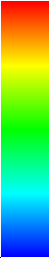
\includegraphics[height=2in]{figures/colormaps/rainbow.png}&
      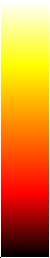
\includegraphics[height=2in]{figures/colormaps/heatmap.png}&         
     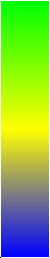
\includegraphics[height=2in]{figures/colormaps/blueYellowGreen.png}&
      
\includegraphics[height=2in]{figures/colormaps/blackGradient.png}&
      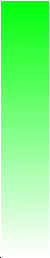
\includegraphics[height=2in]{figures/colormaps/whiteGradient.png}&
      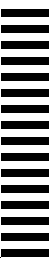
\includegraphics[height=2in]{figures/colormaps/zebra.png}\\
    (a)&(b)&(c)&(d)&(e)&(f)&(g)\\
    \end{tabular}
    \caption{Predefined colormaps: (a) Luminance, (b) Rainbow, (c) Heatmap, (d)  Blue-Green-Yellow, (e) Black Gradient (f) White Gradient (g) Zebra}
    \label{fig:colormaps}
\end{figure}



\begin{figure}[htbp]
\centering
\begin{minipage}[t]{0.48\textwidth}
        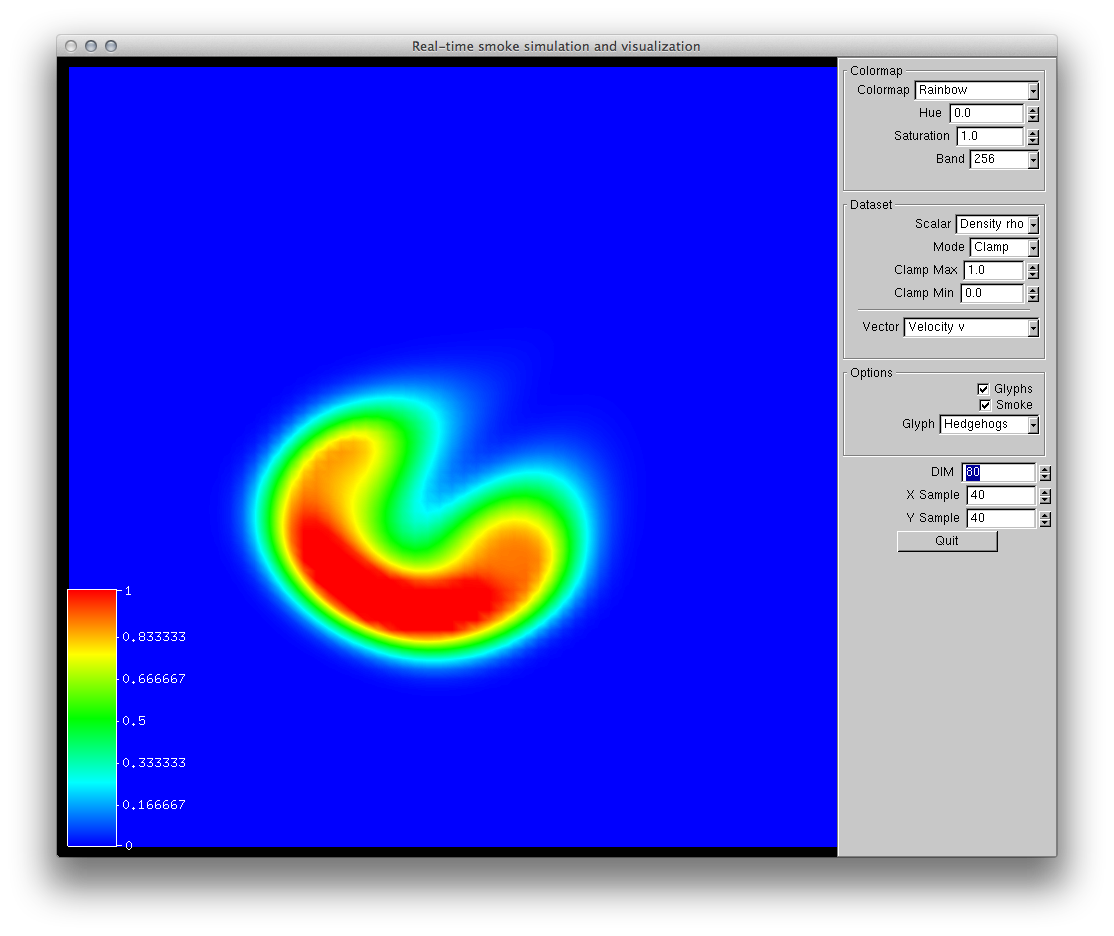
\includegraphics[height=3in]{figures/colormaps/rainbowSmoke.png}
\caption{Fluid density visualized with a rainbow colormap.}
\label{fig:rainbowColormap}
\end{minipage}\hspace{.04\textwidth}%
\begin{minipage}[t]{0.48\textwidth}
        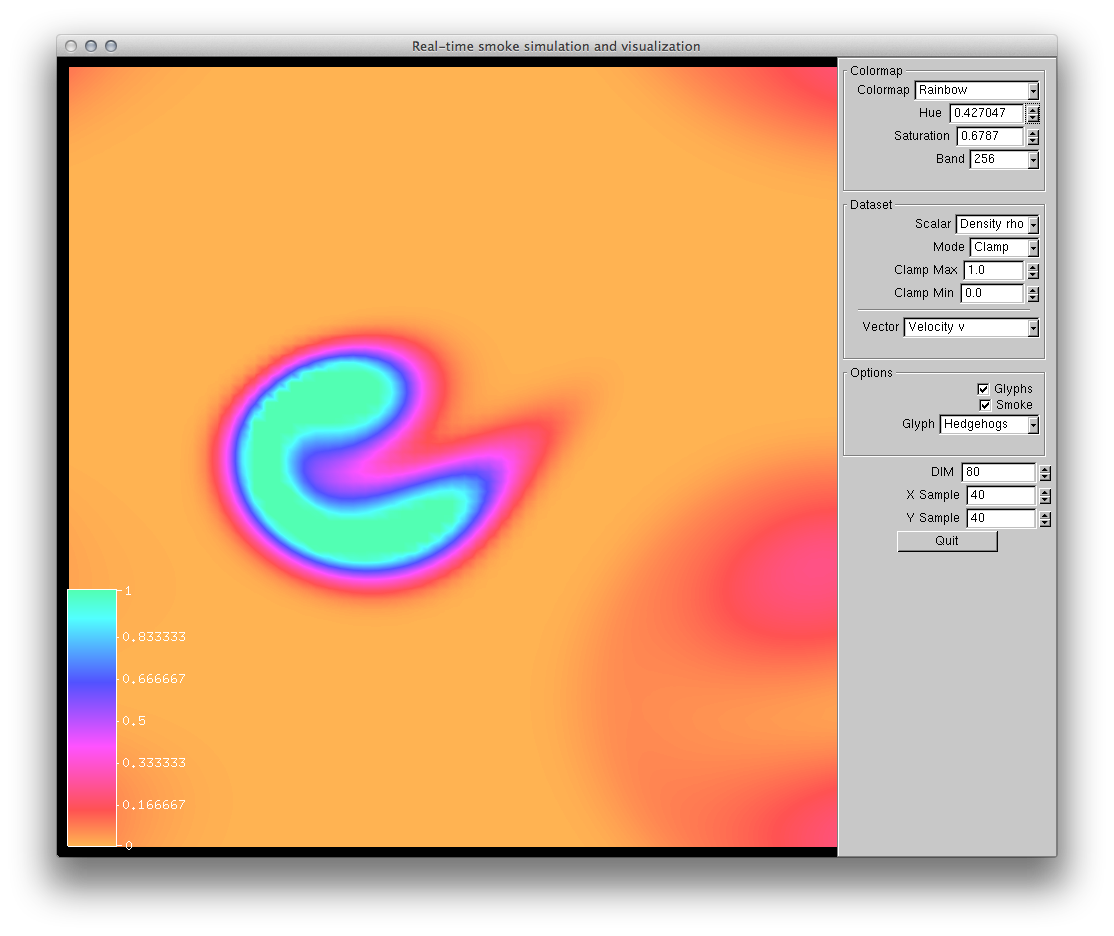
\includegraphics[height=3in]{figures/colormaps/hueAndSaturation.png}
    \caption{Fluid density with a less-saturated and hue-shifted rainbow colormap.}
    \label{fig:saturationAndHueColormap}
\end{minipage}
\end{figure}


\begin{figure}[htbp]
\centering
\begin{minipage}[t]{0.48\textwidth}
        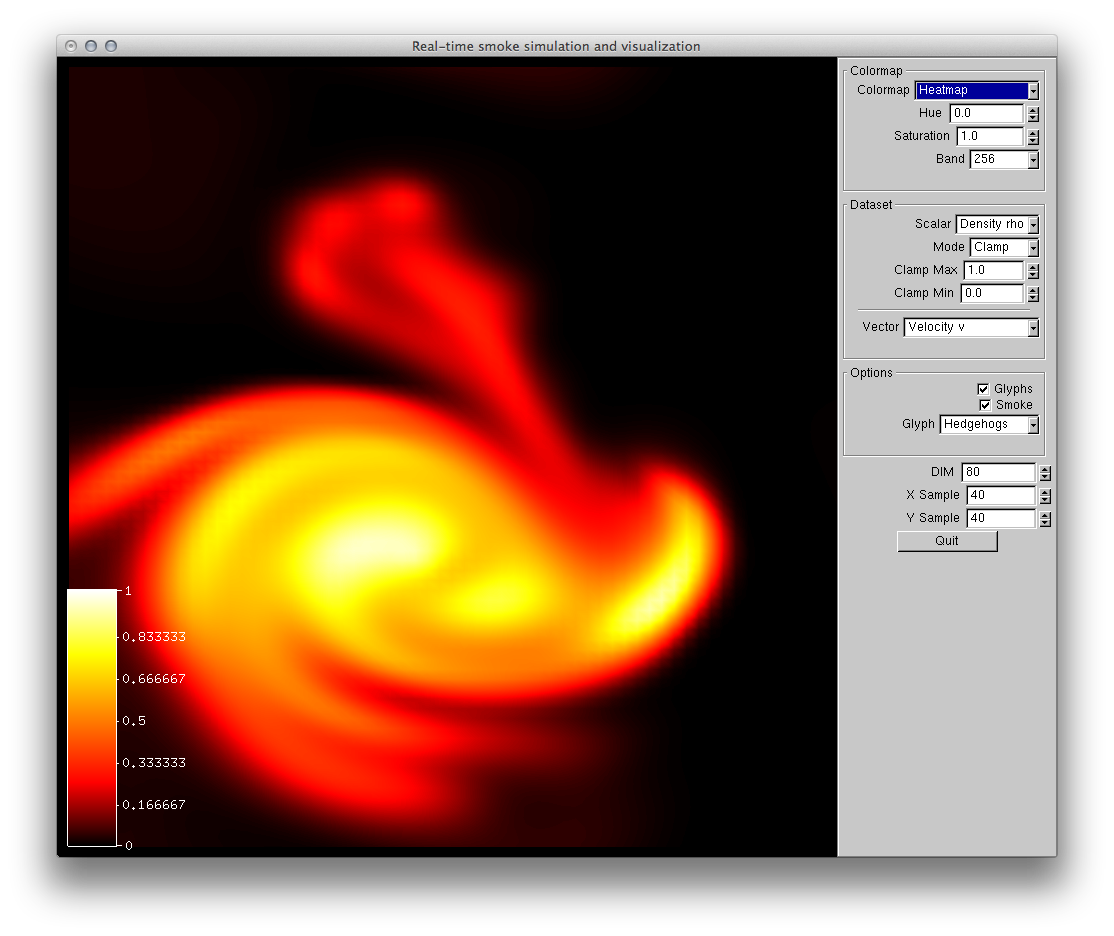
\includegraphics[height=3in]{figures/colormaps/heatmapSmoke.png}
\caption{Fluid density visualized with a heat colormap}
\label{fig:revised:modelingLanguages}
\end{minipage}\hspace{.04\textwidth}%
\begin{minipage}[t]{0.48\textwidth}
        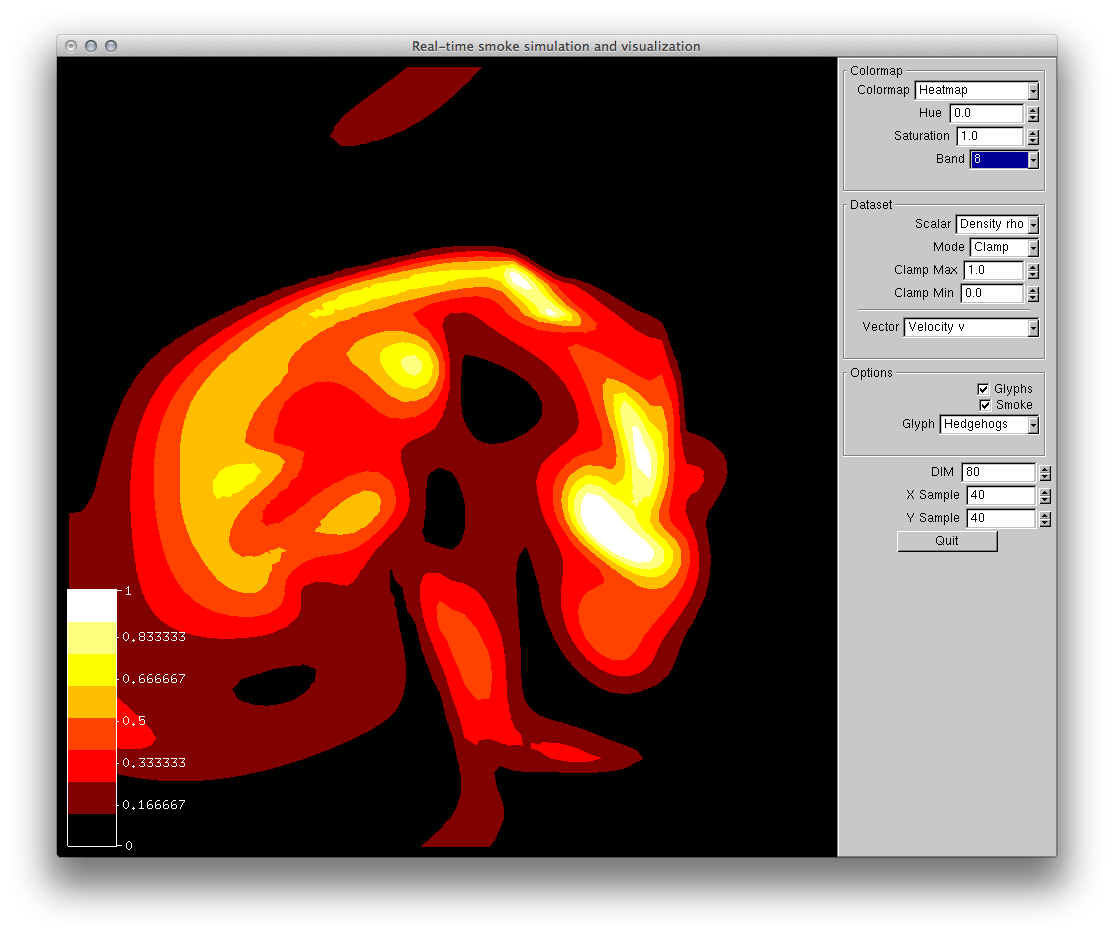
\includegraphics[height=3in]{figures/colormaps/heatmapSmokeBanded.png}
    \caption{Heat colormap with a reduced number of colors. The color banding effect is clearly visible.}
    \label{fig:revised:reqFormat}
\end{minipage}
\end{figure}

\begin{figure}[htbp]
\centering
\begin{minipage}[t]{0.48\textwidth}
        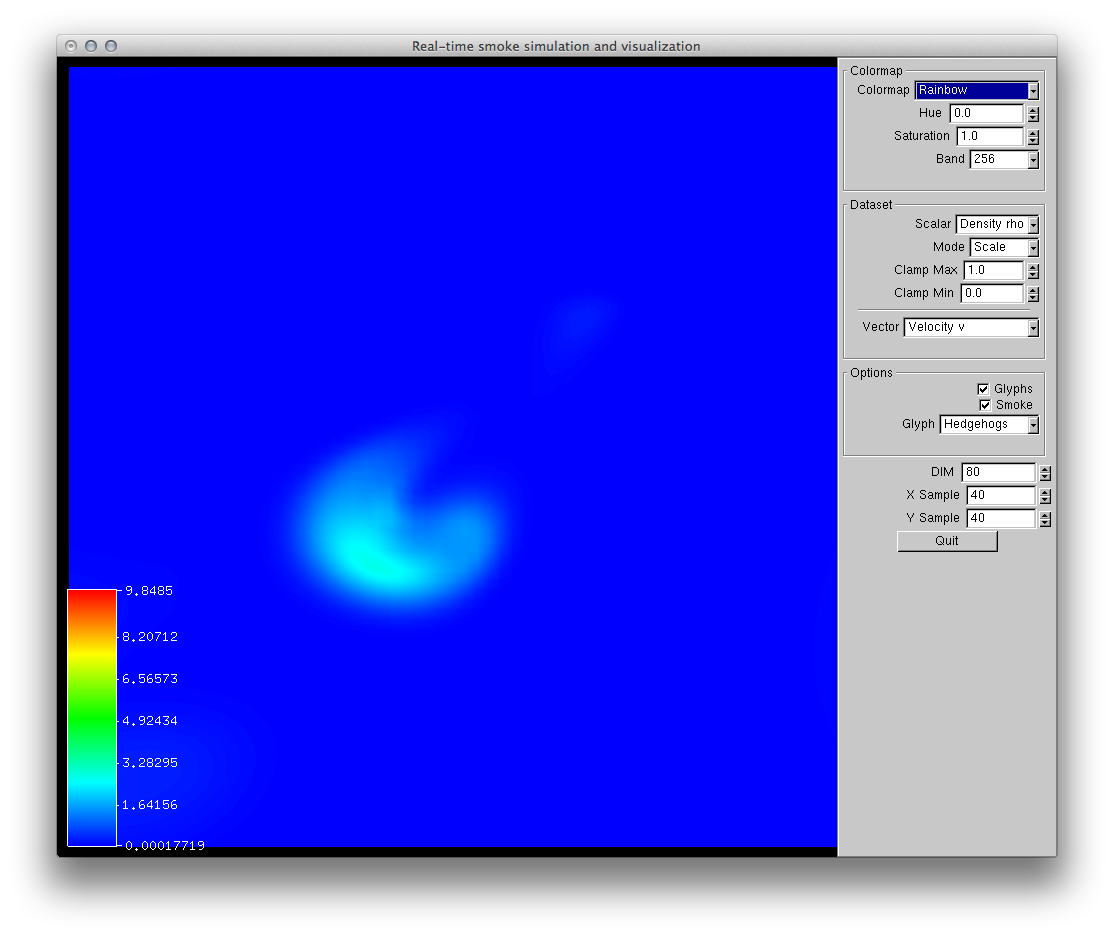
\includegraphics[height=3in]{figures/colormaps/rainbowSmokeScaled.png}
\caption{Scaled valued}
\label{fig:revised:modelingLanguages}
\end{minipage}\hspace{.04\textwidth}%
\begin{minipage}[t]{0.48\textwidth}
        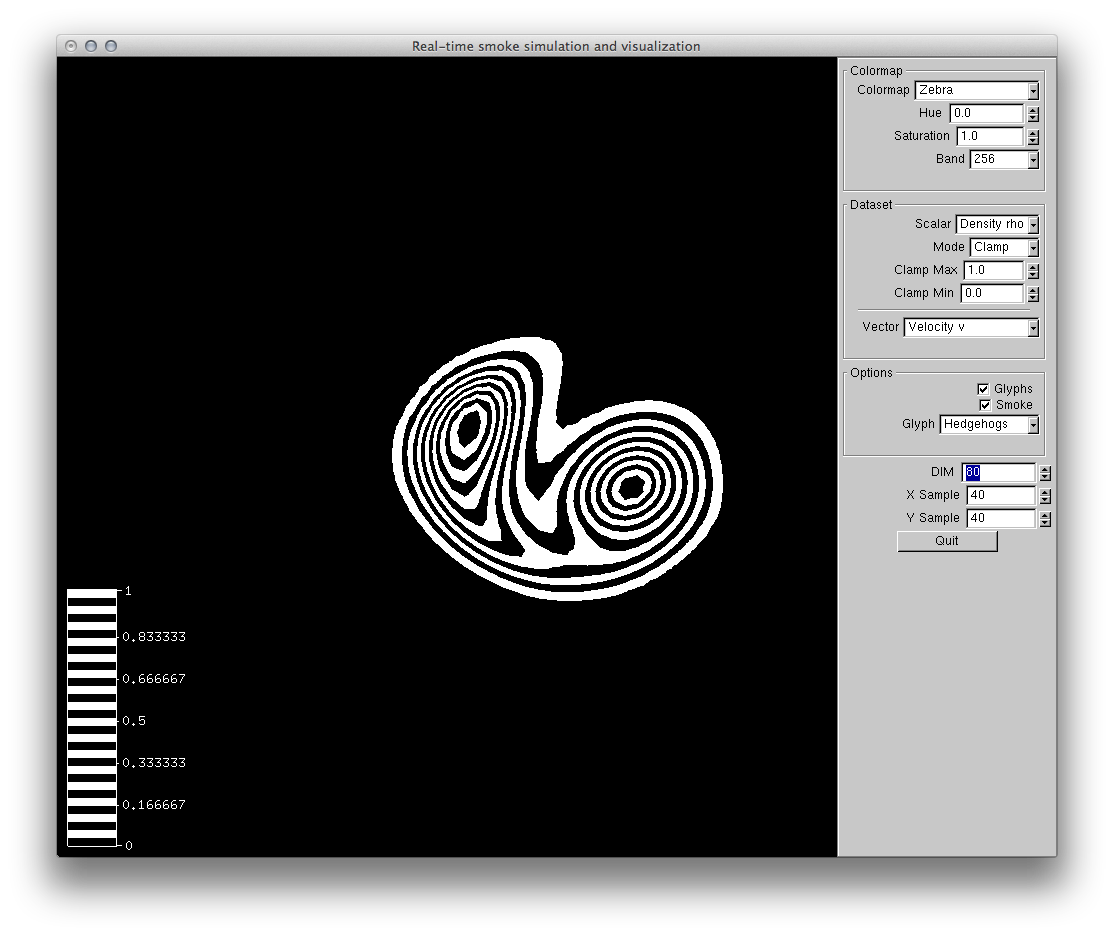
\includegraphics[height=3in]{figures/colormaps/zebraSmoke.png}
    \caption{Density visualized with a zebra colormap that shows areas with high variation.}
    \label{fig:revised:reqFormat}
\end{minipage}
\end{figure}


\subsection{Glyphs}
\subsection{Gradient}
\subsection{Streamlines}
\subsection{Slices}
\subsection{Stream surfaces}